% Chapter 2

\chapter{Rigidity in random graphs} % Main chapter title

\label{Chapter2} % For referencing the chapter elsewhere, use \ref{Chapter1} 

\lhead{Chapter 2. \emph{Rigidity in random graphs}} % This is for the header on each page - perhaps a shortened title

%----------------------------------------------------------------------------------------

The use of the probabilistic method in discrete mathematics has become a prominent idea in the area in recent times. It provide existence proofs where objects have certain desirable properties and it is not always easy to construct explicit examples. This has been just the beginning of the use of probabilistic tools in a deterministic context.

Complex topological spaces arise quite natural in a lot of scientific contexts. Probability theory provides different approaches to model those spaces; even in complex configurations, it can be possible by doing approximations, to study topological invariants. 

In this sense stochastic topology can be thought as a tool for topology in the same sense as statistical mechanics is used to study a macroscopic physical system when the classical mechanics finds these systems very complicated to solve.

Stochastic topology finds its motivation in applied problems. Nevertheless, recent articles have used its techniques to provide probabilistic analogs of very classical topology conjectures, like Whitehead conjecture \cite{Costa15}.

Probability theory can help us to understand the ubiquity of certain mathematical phenomena. For example, \textit{many} simplicial complexes and posets which arise from combinatorial constructions are homotopy equivalent to a wedge of spheres. There is a well-known theorem which states that hiperbolicity is \textit{quite common} in random groups. This means that even under different measures, almost every group is hyperbolic.

We are interested in giving formal meaning to expressions like \textit{"quite common"} or \textit{"many"}.

In this chapter we review rigid expansions in simple probabilistic models. Afterwards, we analyze the feasibility of modeling the curve graph using these proposals.

Familiarity with basic concepts in probability theory such as probability spaces, random variables, and basic theorems will be assumed.

\section{Models for random graphs}

\subsection{The Radó graph}
Let $0 < p < 1$ be fixed, $\G(\N, p)$ consists of all graphs with vertex set $\N$, whose edges are chosen independently and with probability $p$. In other words a random graph $G \in \G(\N,p)$ is a collection $(X_{ij}) = \{ X_{ij} : 1 \leq i < j\}$ of independent $Bernoulli(p)$ r.v., where a pair $ij$ is an edge of $G$ if and only if $X_{ij} = 1$.

Erdös and Rényi proved in \cite[Erdös, Rényi]{RadoUnique}, that every infinite random graph is isomorphic to the \textbf{Radó graph}. This graph have a countably infinite number of vertices, and can be constructed (with probability one) by deciding independently for each pair of its vertices whether to connect them by an edge or not.

A construction of this graph can be done using binary numbers. To do this, identify the vertices of the graph with the natural numbers, then every edge appears between vertices $x$ and $y$ in the graph (assuming $x < y$) whenever the $x$-th bit of the binary representation of $y$ is nonzero. This means, for example, that all odd-numbered vertices will be neighbors of vertex $0$, and that the larger neighbors of vertex $1$ are all vertices with numbers congruent to $2$ or $3$ mod $4$.

\begin{figure}[h!]
	\centering
	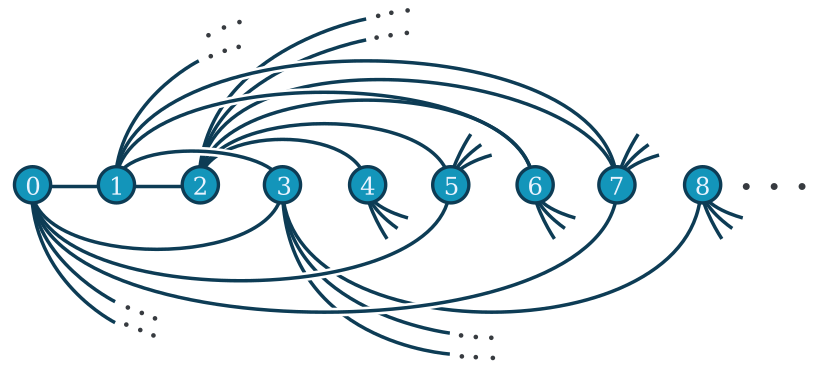
\includegraphics[scale=0.7]{Figures/Rado-graph.png}
	\caption{Binary construction of the Radó graph}
\end{figure}

\subsection{Erdös-Rényi model}
\begin{defini}
We will denote by $\G(n,p)$ to the probability space formed by all the graphs of $n$ vertices and probability measure 
$$ \P(G\in \G(n,p)) = p^{k} (1-p)^{\binom{n}{2}-k} $$
where $k$ is the number of edges in $G$, the $\sigma$-algebra is given by the power set.
\end{defini}

Note: There is a variation of the model where exactly $m$ edges among the $\binom{n}{2}$ possible, are chosen randomly.

We can also think this model like $\binom{n}{2}$ i.i.d. $Bernoulli(p)$ that represent the edges. Using what we know about this r.v. we can immediately get some properties of the degree of a given vertex $v$.

\begin{itemize}
\item The probability that a given vertex $v$ has degree $k$ is given by
$$b(k; n-1,p) = \binom{n-1}{k} \cdot p^{k} \cdot (p-1)^{n-k-1}$$
\item The expected degree is $(n-1)\cdot p$
\item The variance of this degree is $(n-1)\cdot p \cdot (1-p)$
\end{itemize}

The degree distribution can be helpful to do optimizations in the rigid expansions algorithms. In the next chapter we will see how exactly can this be done.

\section{Rigid expansions}

 We will focus in the rigidity calculations for the finite case. Then, we will analyze when $n$ tends to infinite as Radó graph can also be thought as an asymptotic version of the Erdös-Rényi model. For this, we need the calculations of the probability that the following events occur.

\begin{itemize}
\item A vertex $v$ is uniquely determined by $A_{m}$, a set of size $m$
%\item What is the probability that $B_{m}\subset A_{k}$ uniquely determine a vertex $v$ outside of $A_{k}$? (Event $E_2$)
\item A set of size $k$ generate a rigid expansion
\item A set of size $k$ generate a rigid expansion with $s$ new elements
\end{itemize}
\clearpage

For the calculations concerning the first event, take a look to following picture

\begin{figure}[h!]
	\centering
	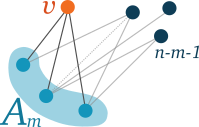
\includegraphics[scale=1]{Figures/uni.png}
	\caption{Probability of uniquely determined vertices}
\end{figure}

If $<A_{m}> = v$ there is a edge between $v$ and every vertex in $A$, and none of the remaining $n-m-1$ vertices is also connected to every vertex in $A$, i.e.
$$\P (E_m) = \P(<A_{m}> = v) = p^{m}(1-p^{m})^{n-m-1}$$
Using the \texttt{networkx} library in \texttt{python} we reproduce the following experiment:
 
\begin{cajita}
\textbf{Uniquely determined vertex experiment} \hfill \break
Fixing $n,p,m$.
\begin{enumerate}
\item Generate an Erdös-Rényi graph $G\in \G(n,p)$ with labeled vertices.
\item Excluding the $n$-th vertex, take a random set of vertices of size $m$.
\item Verify if this random set uniquely determine the $n$-th vertex.
\end{enumerate}
\end{cajita}

In the next chapter we explain how to generate random graphs for the first step. To simplify the process we took, without loosing generality, the last vertex as a particular element of the experiment. When $m=n$ there is no need to do the experiment.

We repeated this experiment 50 times and count the number of times when the random set uniquely determine the $n$-th vertex. Calculating the ratio of the times this happened and the total number of tries, we obtain the empiric probability that a vertex $v$ is uniquely determined by $A_{m}$. 

Fixing $n$ and $p$ we calculate the empiric probability for each possible value of $m$. In the following figure appear the empiric probabilities together with the theoretical calculations.

\clearpage
\begin{figure}[h!]
	\centering
	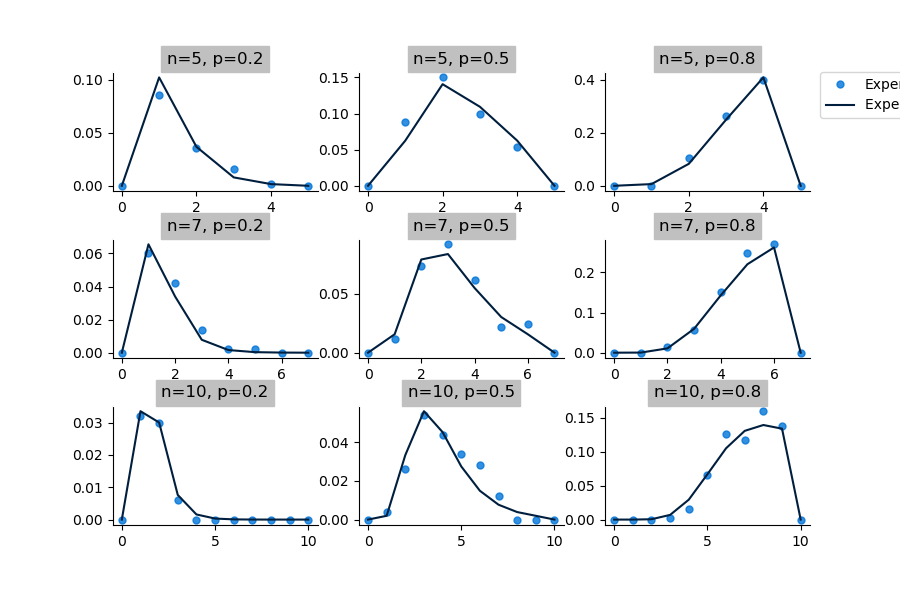
\includegraphics[scale=0.55]{Python/Figures/Uniquely-determinated-fixed-vertex.png}
	\caption{Theoretical and empirical probabilities of uniquely determined a vertex. For different values of $n$ and $p$ varying among all the possible values of $m$}
\end{figure}

Notice that there are certain values of $m$ more \textit{effective} than others, in the sense that, depending on the parameters of the model, it is more likely that a subset of certain size uniquely determine a vertex. This can be used, as outlined in the next chapter, to do optimizations.
 
In following table there is a summary of the maximum of the difference between these two values for distinct values of $n$ and $p$. These values are indicators that the simulations and the calculations describe the same phenomenon.

\bgroup
\def\arraystretch{1.5}%  1 is the default, change whatever you need
\begin{center}
\begin{tabular}{|c|c|c|c|}
\hline
n & 5 & 10 & 15 \\
\hline \hline
 0.2 & 1e^{-8} & 1e^{-8} & 1e^{-8} \\\hline
 0.3 & 1e^{-8} & 1e^{-8} & 1e^{-8} \\\hline
 0.4 & 1e^{-8} & 1e^{-8} & 1e^{-8} \\\hline
\end{tabular}
\caption{Maximums of differences between empirical and theoretical probabilities varying $m$ for different values of $n$ and $p$}
\label{tabla:sencilla}
\end{center}
\bgroup

For the second event, if $A_k$ does not generate a rigid expansion is because none of the subsets of $A_{k}$ determined uniquely a vertex outside of it. We have:
$$\P(A_k \text{ generates a rigid expansion}) = 1 -  \prod_{m=1}^{k} (\rho_{m,k})^{\binom{k}{m}}  $$
where $\rho_{m,k} = \Big(1 -  \P(E_m)\Big)^{n-k}$.

Just as before, we reproduce the following experiment:
 
\begin{cajita}
\textbf{Rigid expansion experiment} \hfill \break
Fixing $n,p,k$.
\begin{enumerate}
\item Generate an Erdös-Rényi graph $G\in \G(n,p)$.
\item Take a random set of vertices of size $k$.
\item Verify if this set generates a rigid expansion
\end{enumerate}
\end{cajita}

Notice that the third step is a critical point in this experiment; we must verify among all the possible subsets of $A_{k}$. In the next chapter we explain the possible optimizations for this part.

Again we repeated this experiment 50 times and calculated the empiric probability that a random set generate a rigid expansion. In the following figure appear empiric and theoretical probabilities for this experiment.

\begin{figure}[h!]
	\centering
	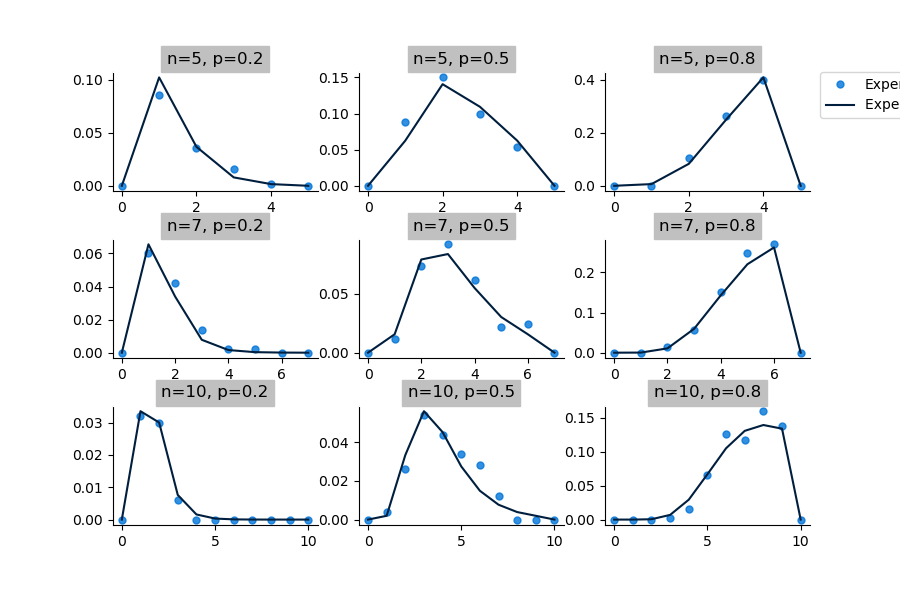
\includegraphics[scale=0.55]{Python/Figures/Uniquely-determinated-fixed-vertex.png}
	\caption{Theoretical and empirical probabilities of uniquely determined a vertex. For different values of $n$ and $p$ varying among all the possible values of $m$}
\end{figure}

The following table let us see that the empirical and theoretical probabilities agree again.

\bgroup
\def\arraystretch{1.5}%  1 is the default, change whatever you need
\begin{center}
\begin{tabular}{|c|c|c|c|}
\hline
n & 5 & 10 & 15 \\
\hline \hline
 0.2 & 1e^{-8} & 1e^{-8} & 1e^{-8} \\\hline
 0.3 & 1e^{-8} & 1e^{-8} & 1e^{-8} \\\hline
 0.4 & 1e^{-8} & 1e^{-8} & 1e^{-8} \\\hline
\end{tabular}
\caption{Maximums of differences between empirical and theoretical probabilities varying $m$ for different values of $n$ and $p$}
\label{tabla:sencilla}
\end{center}
\bgroup

The calculations for the last question are helpful if we want to approximate the sequence of rigid expansions of $A_{k}$ by a Markov chain. Consider $\{0,1, \dots n\}$ as the states space of the Markov chain with transition matrix given by:
$$ a_{k,k+s} = \P(A_{k} \text{ generates a rigid expansion by } s \text{ elements})$$
Notice that, unlike in the stochastic case, the deterministic process stops once a iteration fails to add new vertices. This is because with this approximation we are consider a new $G \in \G(n,p)$ for each step, hence it is allowed to \textit{"have extra tries to expand."}

Unlike past calculations this probability is not that easy to obtain. A first approach to understand this phenomenon is to simulate with our computational tools the following experiment:
 
\begin{cajita}
\textbf{Uniquely determined vertex experiment} \hfill \break
Fixing $n,p,k$.
\begin{enumerate}
\item Generate an Erdös-Rényi graph $G\in \G(n,p)$.
\item Take a random set of vertices $A_{k}$.
\item Produce the first rigid expansion from the graph spanned by $A_{k}$
\item Return the size of the expanded subgraph
\end{enumerate}
\end{cajita}

This experiment yields a random variable which depends on $n, p$ and $k$. Fixing $n$ and $p$ we obtained a sample of size 50 for every possible value of $k$. Using the resulting histogram as an empirical density function we obtain the following figure. It graphically describes the nature of the transition matrix of a sequence of rigid expansions.

\clearpage
\begin{figure}[h!]
	\centering
	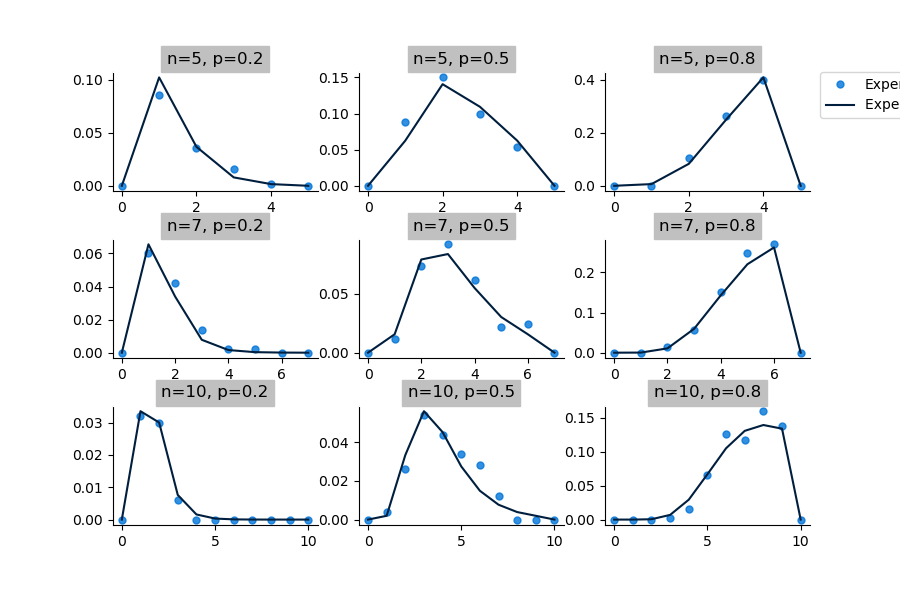
\includegraphics[scale=0.55]{Python/Figures/Uniquely-determinated-fixed-vertex.png}
	\caption{Theoretical and empirical probabilities of uniquely determined a vertex. For different values of $n$ and $p$ varying among all the possible values of $m$}
\end{figure}

Notice that there are certain values of $m$ more \textit{effective} than others, in the sense that, depending on the parameters of the model, it is more likely that a subset of certain size uniquely determine a vertex. This can be used, as outlined in the next chapter, to do optimizations.
 
In following table there is a summary of the maximum of the difference between these two values for distinct values of $n$ and $p$. These values are indicators that the simulations and the calculations describe the same phenomenon.

\bgroup
\def\arraystretch{1.5}%  1 is the default, change whatever you need
\begin{center}
\begin{tabular}{|c|c|c|c|}
\hline
n & 5 & 10 & 15 \\
\hline \hline
 0.2 & 1e^{-8} & 1e^{-8} & 1e^{-8} \\\hline
 0.3 & 1e^{-8} & 1e^{-8} & 1e^{-8} \\\hline
 0.4 & 1e^{-8} & 1e^{-8} & 1e^{-8} \\\hline
\end{tabular}
\caption{Maximums of differences between empirical and theoretical probabilities varying $m$ for different values of $n$ and $p$}
\label{tabla:sencilla}
\end{center}
\bgroup


\section{Radó graph as a model for the curve graph}
The Radó graph satisfy that every finite or countably infinite graph is an induced subgraph of it \cite{DarReferenciaAqui1}. Notice that if we have a surface $S$ of finite genus is not possible that the Radó graph is embedded into $C(S)$. This because of the restriction in the clique number of $C(S)$. Not only that, it turns out that the converse is also valid; this is claimed in the following result by Bering and Gaster \cite{beringGaster}.

\begin{theorem}
The random graph embeds into the curve graph $C(S)$ of a surface $S$ if and only if $S$ has infinite genus.
\end{theorem}

Therefore, if we want to study the curve graph of a surface of finite genus using the Radó graph, we have to think it as a subgraph of it. A simple but naive approach to do it is to take a random subset of vertices of a graph $G\in \G(\N, p)$, then consider the vertex induced subgraph. It turns out that for a.e. $G\in \G(\N, p)$ the sequence $cl(G_n)$ is almost entirely determined.

\begin{theorem}
For a.e. $G \in \G(\N,p)$ there is a constant $m_0 = m_{0}(G)$ such that if $n \geq m_o$ and $n'_{r} \leq n \leq n_{r+1}$, then $cl(G_{n}) = r$.
\end{theorem}

Notice that if $r$ is a fixed finite number the number for vertices should be finite as well. Therefore, we will not be able to build the curve graph by an uniform selection of vertices. 

The problem is that the curve graph has a very specific clique number. Unlike the other properties listed above, this is the only one which seems not generic and that actually depends on the genus of the surface.

This is not the first time that a complication like this appear in the literature, for example, in \cite{Alcazar15}) they want to ensure that the random graph doesn't have cycles (in this case it's implied that the clique number is 2). A discrete MCMC algorithm was used to sample uniformly random trees of size $n$, with the \texttt{generate algorithm}. It produce a maximal tree of any not directed graph with $n$ vertices taken uniformly among all the possibles ones. In the appendix we summarize the results of this method, for a deeper analysis look at \cite{Broder89}.

Even if we can provide an analog of the generate algorithm which ensure any other fixed clique number, the idea is to study rigid expansions in a simpler probabilistic approach. In this spirit it remains to examine the plausibility of the Erdös-Rényi model.

\section{Erdös-Rényi as a model for the curve graph}
In chapter one, we settled the bases to model the curve graph associated to any given surface. Summarizing the results, we're looking to couple the exposed models in a way that we can guarantee the following properties:

\begin{enumerate}
\item Countably infinite number of vertices
\item Connectedness
\item Locally infinite
\item Clique number $3g-3+m$
\item Infinite diameter
\end{enumerate}

\subsection{Connectivity}
\begin{theorem}
Let $\omega(n)$ be a function that tends to infinity arbitrarily slow as $n$ tends to infinity
\begin{itemize}
\item If $p\geq \frac{log(n)+ \omega(n)}{n}$ then 
$$\lim_{n \to \infty} \P(G \in \G(n,p) \text{ is connected}) = 1$$
\item If $p\leq \frac{log(n)- \omega(n)}{n}$ then
$$\lim_{n \to \infty} \P(G \in \G(n,p) \text{ is disconnected}) = 1$$
\end{itemize}
\end{theorem}
 
This can be proven by first showing that for a large $n$ almost all graphs consists of a connected graph having $n-k$ effective vertices and $k$ isolated points, the theorem follows from a counting argument. The complete proof can be found in \cite[Erdös-Rényi, 59]{OnRandomGraphs}.
 
\subsection{Locally infinity}

We already discuss that $deg(v)$ behaves like a binomial random variable. So we just have to describe $p$ so that a.a.s $deg(v)$ tends to infinite along with $n$. Consider $v\in V(G(n+1,p))$, so:
$$ \P(deg(v)=k) = \binom{n}{k} \cdot p^{k} \cdot (1-p)^{n-k}$$
Let $\epsilon>0$ and $a>0$ be fixed, taking $p=\frac{\epsilon}{n^{a}}$ we have
\begin{center}
\begin{tabular}{ r l }
 $\displaystyle\lim_{n\to \infty } \P(deg(v)=k) =$ & $\displaystyle\lim_{n\to \infty} \binom{n}{k} \cdot \left( \frac{\epsilon}{n^a} \right)^k \cdot \left( 1-\frac{\epsilon}{n^a}\right)^{n-k}$ \\
 $\sim$ &  $\displaystyle\lim_{n\to \infty} \frac{n^k}{k!}\cdot  \frac{\left(\frac{\epsilon}{n^a}\right)^k} {\left(\frac{n^a - \epsilon}{n^a}\right)^k} \cdot \left(1-\frac{\epsilon}{n^a}\right)^{n} $\\
$=$ &  $\displaystyle\lim_{n\to \infty} \frac{n^k}{k!}\cdot \left(\frac{\epsilon} {n^a - \epsilon}\right)^k \cdot \left(1-\frac{\epsilon}{n^a}\right)^{n} $\\
\end{tabular}
\end{center}
the last term of this expression have a very interesting asymptotic behavior, when $a=1$ we already know that $\left(1-\frac{\epsilon}{n^a}\right)^{n} \to e^{-\epsilon}$ which actually determine the Poisson approximation of the Binomial random variable. When $a\neq 1$ then we have to do the following analysis
$$\displaystyle\lim_{n\to \infty } \left( 1 - \frac{\epsilon}{n^a}\right)^n = \displaystyle\lim_{n\to \infty} exp\left( ln \left( 1 - \frac{\epsilon}{n^a}\right)^n\right) = \displaystyle\lim_{n\to \infty} exp\left(n \cdot ln \left( 1 - \frac{\epsilon}{n^a}\right)\right)$$
So we need to study $\displaystyle\lim_{n\to \infty} f(n) = \displaystyle\lim_{n\to \infty} n \cdot ln \left( 1 - \frac{\epsilon}{n^a}\right)= \displaystyle\lim_{n\to \infty}\frac{ln \left( 1 - \frac{\epsilon}{n^a}\right)}{\frac{1}{n}}$, using L'ôpital's rule for limits we obtain:
$$\displaystyle\lim_{n\to \infty } f(n) = 
\displaystyle\lim_{n\to \infty } \frac{\frac{1}{\left( 1 - \frac{\epsilon}{n^a}\right)}\cdot (\epsilon a n^{-a-1})}
{-1\cdot n^{-2}} = 
\displaystyle\lim_{n\to \infty } \frac{\frac{n^a}{n^{a} - \epsilon}\cdot (\epsilon a n^{-a-1}) \cdot {n^{2}}}{-1} = 
\displaystyle\lim_{n\to \infty } - \frac{\epsilon a n}{n^{a} - \epsilon} =
\displaystyle\lim_{n\to \infty } - \frac{\epsilon a}{a n^{a-1}}
$$
from here we can see that if $a>1$ then $\displaystyle\lim_{n\to \infty } f(n) = 0$ and if $a<1$  then $\displaystyle\lim_{n\to \infty } f(n) = -\infty$
Notice that $\P(deg(v)=0) = \left(1 - \frac{\epsilon}{n^a} \right)^n$, so:
$$ \displaystyle\lim_{n\to \infty} \P\left(deg(v)=0\right) = \begin{cases} 
\displaystyle\lim_{n\to \infty}e^{f(n)} = 1, & \mbox{if } a>1 \\ 
\displaystyle\lim_{n\to \infty}e^{f(n)} = 0, & \mbox{if } a<1 \end{cases} $$

Another perspective to study the degree of vertices is to consider $X_{k} = X_{k} (G)$, the random variable that describes the number of vertices of degree $k$ in a graph $G$. The following theorem gives a describe this invariant.

\begin{theorem}
Let $\epsilon>0$ be fixed, $\epsilon n^{-3/2} \leq p = p(n) \leq 1 - \epsilon n^{-3/2}$, let $k = k(n)$ be a natural number and set $\lambda_{k} = \lambda_{k}(n) = n\cdot b(k;n - 1,p)$. Then the following assertions hold.

\begin{itemize}
\item If $\lim \lambda_{k}(n) = 0$, then $\lim P(X_{k} = 0) = 1$. 
\item If $\lim \lambda_{k}(n) = \infty$, then $\lim P(X_{k} > t) = 1$
for every fixed $t$.
\item If $0 < \lim\lambda_{k}(n) < \lim \lambda_{k}(n) < \infty$,
then $X_{k}$ has asymptotically Poisson distribution with mean $\lambda_{k}$: 
$$P(X_{k} = r) \sim e^{\lambda_{k}}\cdot \lambda_{k}^{r}/ r!$$
for every fixed $r$.
\end{itemize}
\end{theorem}

The hypothesis on $ p $ appears when we consider a loose upper bound on the expected degree of $ X_ {k} $, using this bound we can directly assert that if $ pn ^ {2} \ to \ infty $ then almost every $ G \ in G (n, p) $ consist of independent edges and isolated vertices. The complete argument of this claim among with the proof of the theorem can be found in \cite[Bollobás, p.61]{Bollobas}.

If $k$ is a finite fixed number, then the past theorem is saying that when $\lim \lambda_{k}(n) = 0$ then a.a.s there aren't vertices of finite degree. In the second case we obtain that there are as many vertices with degree $k$. And in the third case we can describe explicitly the degree distribution, which concentrate the degree in a finite range around the mean $\lambda_{k}$. So to fit the model into the context of the curve complex we need to choose $p = p(n)$ so that the first case is satisfied for any fixed $k$ i.e.
$$\lambda_{k} = n \binom{n-1}{k} p^{k} (1-p)^{n-k-1} \to 0$$

\subsection{Clique number}

%Let $X_r$ denote the random variable which counts the number of $r-$cliques in a graph $G$. We have
%$$E_{r} = E(X_r) = \binom{n}{r}p^{\binom{r}{2}}$$
%Let $r_0 = r_0(n,p)$ be the positive real number satisfying
%$$f (r_0) = (2\pi)^{- 1/2} n^{n+ 1/2} (n - r_0)^{-n+r_0-1/2} r_0^{-r_0- 1/2} p^{r_0(r- 1)/2} =1$$
%$f(r)$ is the expression for $E_r$ replacing $\binom{n}{r}$ with its Stirling approximation.
%It is easily checked that
%\begin{center}
%\begin{tabular}{ r l }
%$r_0$ & $ = 2 \text{log}_{b}(n) - 2 \text{log}_{b} \text{log}_{b}(n) + 2 \text{log}_{b}(e/ 2) + 1 + o(1)$ \\
%& $= 2 \text{log}_{b}(n) + O(\text{loglog} (n))$\\
%& $= \frac{2log(n)}{log(b)} + O(\text{loglog}(n))$
%\end{tabular}
%\end{center}

%to simplify the notation, let $b=1/p$.

%Let $0<\epsilon<\frac{1}{2}$. Given a natural number $r \geq 2$, let $n_r$ be the maximal natural number for which
%$$E(n_r, r) \leq r^{-(1+\epsilon)}$$
%and let $n'_{r}$ be the minimal natural number for which
%$$E(n'_{r}, r)\geq r^{1+\epsilon}$$


Let $X_r$ be the random variable that counts the number of complete $r-$graphs in a graph $G$. We have
$$E_{r} = E(X_r) = \binom{n}{r}p^{\binom{r}{2}}$$
Using again the Stirling approximation for $\binom{n}{r}$ we have
$$E_{r} = (2\pi)^{- 1/2} n^{n+ 1/2} (n - r)^{-n+r-1/2} r^{-r-1/2} p^{r(r- 1)/2}$$
The premise of proposing the ER Model is that it is necessary to do a asymptotic analysis. If $r$ is a fixed finite number we obtain
$$\lim E_{r} = C_{r} \cdot p(n)^{\lambda_{r}}$$
where $C_{r}$ and $\lambda_{r}$ are fixed finite constants. To guarantee a finite clique number it is required that $E_{r+1} \to 0$ and simultaneously $E_{r+1} \to \infty$ but this is contradictory.

Again, this property interfere with the proposed model, but we can still provide an analogue of Bering and Gaster result.

Let $Y_{r}$ be the random variable that counts the number of $r-$cliques.
$$\E(Y_{r}) = \binom{n}{r} \cdot (1-p^{r})^{n-r} \cdot p^{\binom{r}{2}}  $$

\begin{theorem}
Let $r = r(n) = O(n^{1/3})$ and let $p=p(n)$, $0<p<1$, be such that
$$\binom{n}{r} p^{\binom{r}{2}} \to \infty \text{ and } \binom{n}{r+1} p^{\binom{r+1}{2}} \to 0 $$
Then a.e $G_{p}$ has clique number $r$
\end{theorem}
The second condition on $p$ implies that almost no $G_{p}$ contains a $K^{r+1}$ so $cl(G_{p})\leq r$ asymptotically almost surely. The first condition on $p$ is simply that $\E (Y_{r}) \to  \infty$. The idea to proof this theorem is to use the calculations for $\E(Y_{r})$ and a first moment argument will work for the rest of the argument. A full proof can be find in \cite[Bollobás, p.290]{Bollobas}.

It is implicit in the theorem that the clique number tends the infinity. Due that $r=3g-3+m$ this implies that the curve graph corresponds to a surface whether of infinite diameter or with an infinite number of punctures.

\subsection{Diameter}

The diameter of a graph $G$, denoted by $diam(G)$, is the maximal distance between pairs of vertices of $G$.

For surfaces of finite genus we should had ensure infinite diameter. In \cite[Bollobás, p.259]{Bollobas} we can find theorems that describe the conditions under this can be done. By the past results now we must guarantee that the diameter is equal to 2, so the model match the properties of curve graphs for infinite genus surfaces.

%This means that if we want to have infinite diameter, we need that $d$ tends to infinity as $n$ does, while the condition $pn/(log\text{ }n)^{3} \to \infty$ is also satisfied i.e.
%$$ \frac{(n\cdot\text{log}(n^{2}/c))^{1/d}}{(\text{log n})^{3}} \to \infty$$

\begin{theorem}
If $p$ is taken fixed $G(n,p)$ has diameter 2 with high probability 
\end{theorem}

\begin{proof}
Consider the random variable $X_{n}$ which is the number of vertex pairs in a graph in $\G(n,p)$ with no common neighbors. By Markov's inequality we have that

$$\P(X_{n} \geq 1)\leq \E(X_{n}) = \binom{n}{2} \cdot \P(\text{two vertices doesn't have common neighbors}) = \binom{n}{2} (1-p^{2})^{n-2}$$

which tends to zero as $n\to \infty$
\end{proof}



%In the first chapter we mention that 
%That's why it's worth to enunciate the following theorem which can be found in \cite[Khale, 16]{Khale}.
%\begin{theorem}
%Let $k \geq 3$ and $\epsilon > 0$ be fixed. If
%$$\left(\frac{(C_{k} + \epsilon \text{log } n} {n} \right) n^{1/k} \leq p \leq \frac{n^{-\epsilon}}{n^{1/(k+1)+\epsilon}}$$
%where $C_{3} = 3$ and $C_{k} = k/2 + 1$ for $k > 3$, then w.h.p. $X$ is rationally homotopy equivalent to a bouquet of $k$-dimensional spheres.
%\end{theorem}

%We can use the Erdös-Rényi model to obtain random simplicial complexes through clique complexes. The clique complex or flag complex $X(G)$, of a graph $G$ is the simplicial complex with all complete subgraphs of $G$ as its faces. The 1-skeleton of $X(G)$ is $G$ itself. $X(G(n, p))$ will be abbreviated by $X(n, p)$ for now on.
%The main remaining conjecture for the topology of random clique complexes is that these rational homotopy equivalences are actually homotopy equivalences.

%\begin{conje}
%The bouquet-of-spheres conjecture.
%Let $k \geq 3$ and $\epsilon > 0$ be fixed. If
%$$\frac{n^{\epsilon}}{n^{1/k}} \leq p \leq \frac{n^{-\epsilon}}{n^{1/(k+1)}}$$
%then w.h.p. $X$ is homotopy equivalent to a bouquet of $k$-spheres.
%\end{conje}